\documentclass{standalone}
\usepackage{pgfplots}
\pgfplotsset{compat=1.15}
\usetikzlibrary{calc,hobby,arrows.meta,3d}

\usepackage{xcolor}
\definecolor{morange}{RGB}{255,127,14}
\definecolor{mblue}{RGB}{31,119,180}
\definecolor{mred}{RGB}{214,39,40}
\definecolor{mpurple}{RGB}{148,103,189}
\definecolor{mgreen}{RGB}{44,160,44}

\begin{document}
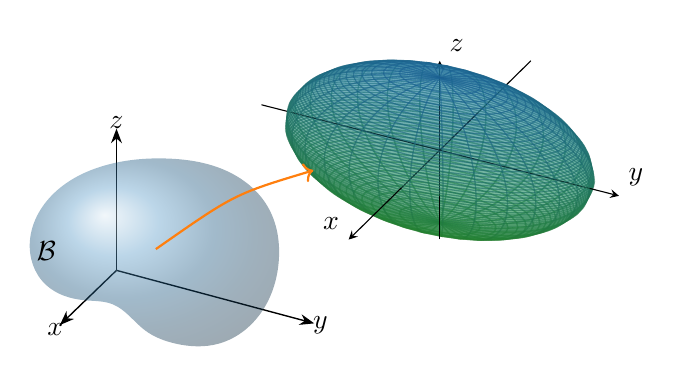
\begin{tikzpicture}[
scale=.1,
every pin/.style={inner sep=1pt},
every pin edge/.style={black},
line width=.5pt,
axisProp/.style={x={(-136:2cm)},
y={(-15:2cm)},
z={(90:2cm)}},
axis/.style={x={(-136:2cm)},
y={(-15:4.5cm)},
z={(90:3cm)}}]
\begin{axis}
    [view={117}{30},
    scale=10,
    xshift=20cm,
    yshift=10cm,
    colormap={slategraywhite}{rgb255=(44, 160, 44) rgb255=(31, 119, 180)},
    %color = mgreen;
    axis lines=center, axis on top,ticks=none,
    set layers=default,axis equal,
    xlabel={$x$}, ylabel={$y$}, zlabel={$z$},
    xlabel style={anchor=south east},
    ylabel style={anchor=south west},
    zlabel style={anchor=south west},
    enlargelimits,
    tick align=inside,
    domain=0:2.00,
    samples=30, 
    z buffer=sort,
    ]
    \addplot3 [surf,opacity=0.4,domain=-1:0, domain y=0:360] ({sin(y)*sqrt(1-x^2)},{2*cos(y)*sqrt(1-x^2)},{x});
    \addplot3 [surf,opacity=0.4,domain=0:1,
    domain y=0:360,on layer=axis foreground] ({sin(y)*sqrt(1-x^2)},{2*cos(y)*sqrt(1-x^2)},{x});
    \end{axis}
\begin{scope}[shift={(-5,-2.7)},axisProp,>=Stealth]
\draw[->] (0,0,0) -- (5,0,0);
\node at (5.4,0,0) {$x$};
\draw[->] (0,0,0) -- (0,13,0);
\node at (0,13.4,0) {$y$};
\draw[->] (0,0,0) -- (0,0,9);
\node at (0,0,9.4) {$z$};
\end{scope}
\shade[ball color=mblue!, closed hobby, opacity=.4] plot coordinates 
{(15.6,-1.6) (14.2,5.4) (8.1,10.3) (1.5,11.5) (-6.2,10.7) (-12.5,7.5) (-16,1)
 (-14,-4.5) (-9,-6.5) (-5.5,-7) (-1.4,-10.3) (2.5,-12) (8,-12) (13.8,-7.4)};
\node at (-13.9,-0.3) {$\mathcal{B}$};
\begin{scope}[shift={(0.0,0.0)},
axis]
\end{scope}
\node at (35, 0, -70) {};
\draw[->, morange, thick] (0, 0, 0) .. controls (10, 7, 0) .. (20, 10, 0);
\end{tikzpicture}
\end{document}